\subsection{3ra etapa: Retransmisiones en función del delay en los ACK's}

En esta etapa de la experimentación analizamos la variación de la cantidad de retransmisiones enviadas entre el cliente
y el servidor en función del delay.
Para mantener el experimento bajo condiciones lo más controladas posibles (pero intentando no olvidar el hecho de que
simulamos una red local real), decidimos fijar el valor $ACK\_CHANCE=0.95$. Descartar un paquete obliga necesariamente 
a la retransmisión del mismo, y esto es independiente del delay que utilicemos ya que queda determinado por la
''tirada de la moneda''. Sin embargo, consideramos que un 95\% de probabilidades de que el paquete sea enviado con éxito se aproxima bastante a la realidad y no impacta en gran medida a la experimentación.

Al mismo tiempo fijamos el paquete del tama\~no enviado en 50 KB, ya que es un valor lo suficientemente grande como 
para que deba ser transmitido en varias partes, pero al mismo tiempo lo suficientemente peque\~no como para poder
repetir el experimento varias veces sin esperar demasiado.

Mantuvimos el valor por default de las siguientes constantes: 
\begin{itemize}
\item{RETRANSMISSION\_TIMEOUT: 0.5 }
\item{MAX\_RETRANSMISSION\_ATTEMPTS: 5 }
\item{RECEIVE\_BUFFER\_SIZE: 1024}
\end{itemize}

Finalmente, el delay en el envío de los ACK's es generado tanto del lado del cliente como del servidor.

Los resultados son mostrados en 3 gráficos distintos ya que resulta muy interesante el impacto del delay en relación al
valor de retransmission timeout y max retransmission attempts.
Para valores de delay peque\~nos la cantidad de retransmisiones fue peque\~na también, y en casi todos los casos
producto de una tirada de la moneda fallida, lo que llevó al paquete a ser descartado (Notemos que 
incluso para un delay = 0,
uno de los paquetes tuvo que ser descartado). 
Al enviar los paquetes que contiene ''payload'', el cliente espera recibir un ACK
por parte del server en un tiempo menor o igual que RETRANSMISSION\_TIMEOUT. Por este motivo, al ser el delay menor
a este valor, en ningún momento forzamos al cliente a retransmitir sus paquetes.

\begin{figure}[H]
	\begin{center}
		  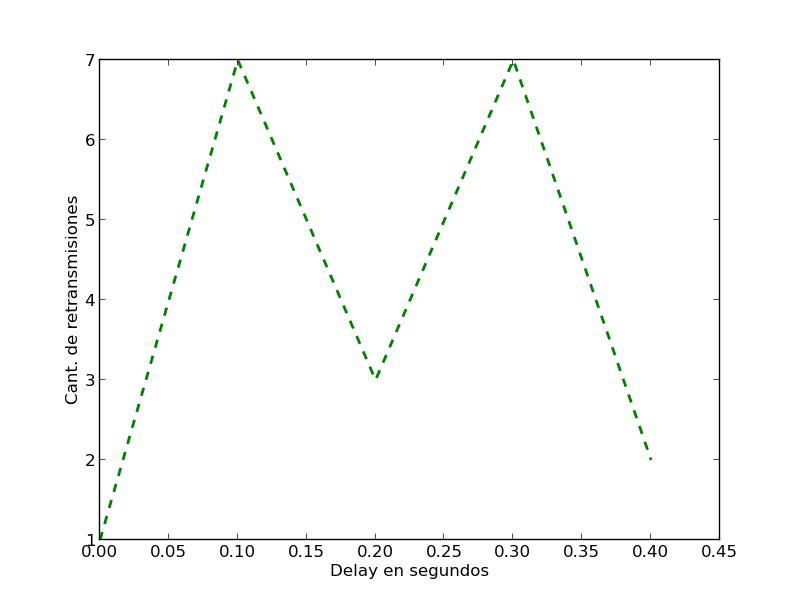
\includegraphics[scale=0.40]{../graficos/retransmissions_1.png}
		  \caption{Delays tomados en un intervalo entre 0 y RETRANSMISSION\_TIME\_OUT }
		  \label{fig:contra1}
	\end{center}
\end{figure}

~

En esta etapa de la experimentación podemos observar cómo el valor del delay impacta linealmente en la cantidad de
retransmisiones que deben realizarse, lo cual es bastante lógico. Si el delay del ACK por parte del server es 1.5 (3
veces mayor al retransmission timeout), es de esperar que el paquete sea retransmitido entre 3 o 4 veces antes de que
sea recibido. Lo mismo con cada múltiplo del timeout(0.5) entre 1 y 5, con lo cual nuestro intervalo de análisis de
delay quedaría delimitado por 0.5 - 2.5 . Decidimos extender el límite superior hasta 3 para ver qué sucedía en los
casos borde, ya que se corre el riesgo de superar el valor MAX\_RETRANSMISSION\_ATTEMPTS y forzar la finalización
del intercambio, tal como indica el protocolo.

\begin{figure}[H]
	\begin{center}
		  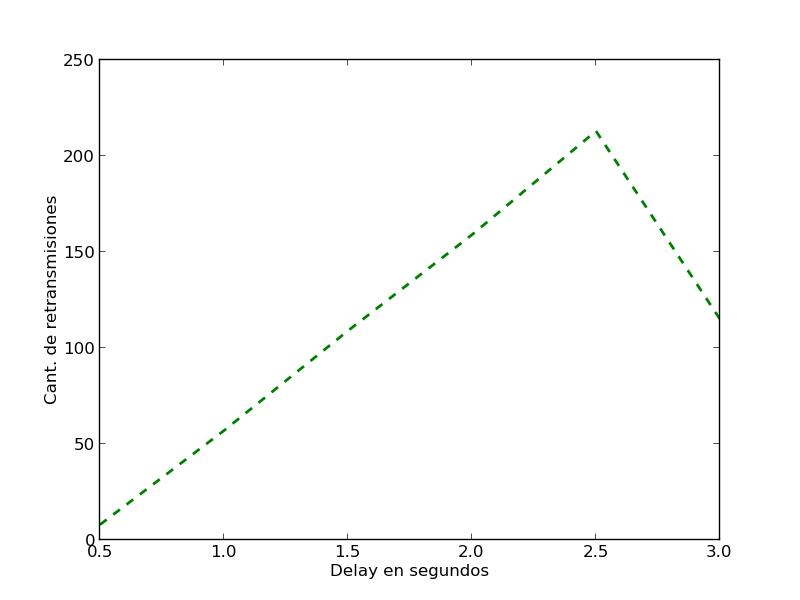
\includegraphics[scale=0.40]{../graficos/retransmissions_2.png}
		  \caption{Delays tomados entre R\_TIME\_OUT y 6*R\_TIME\_OUT}
		  \label{fig:contra1}
	\end{center}
\end{figure}

Efectivamente, para un delay de 3 segundos se producen solo 115 retransmisiones debido a que el límite fue superado.
Si a la demora producida por el delay le sumamos la posibilidad de que el paquete sea descartado por la tirada fallida
de una moneda, resulta muy probable que el límite de retransmisiones sea alcanzado en los casos de borde.

~

\begin{figure}[H]
	\begin{center}
		  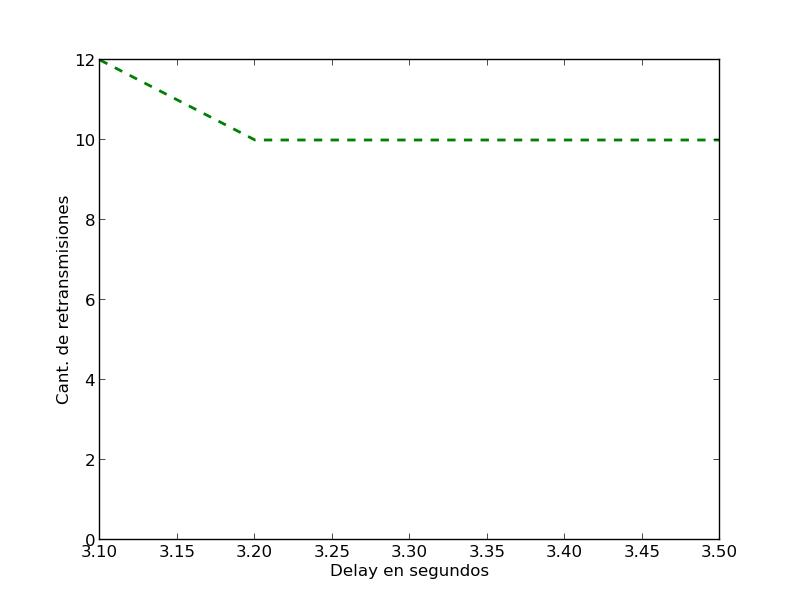
\includegraphics[scale=0.40]{../graficos/retransmissions_3.png}
		  \caption{Valores mayores a 6*R\_TIME\_OUT}
		  \label{fig:contra1}
	\end{center}
\end{figure}

Finalmente para valores de delay superiores a 

RETRANSMISSION\_TIME\_OUT * (MAX\_RETRANSMISSION\_ATTEMPTS + 1), 

el número máximo es superado con los primeros paquetes, lo que explica un número bajo de retransmisiones debido
a la terminación inesperada del intercambio. Tanto cliente como servidor liberar sus recursos al no obtener respuestas.
